\item \textbf{{[}DHS/PRELIM/9597/2018/P1/Q3{]} }

A linked list Abstract Data Type (ADT) has the following operations
defined: 
\begin{itemize}
\item \texttt{Create()} -{}- creates an empty linked list; 
\item \texttt{Insert(item, p)} -{}- inserts new value, \texttt{item}, into
linked list so that it is at position \texttt{p} in the linked list.
Assume that the linked list contains at least \texttt{(p - 1)} items
before the insertion. 
\item \texttt{Delete(p)} -{}- deletes the item at position \texttt{p} in
the linked list; 
\item \texttt{Length()} -{}- returns the number of items in the linked list; 
\item \texttt{IsEmpty()} -{}- returns \texttt{True} if linked list is empty; 
\item \texttt{IsFull()} -- returns \texttt{True} if linked list is full; 
\end{itemize}
The linked list is implemented by the use of a collection of nodes
that have two parts: the item data and a pointer to the next item
in the list. In addition there is a \texttt{Start} pointer which points
to the first item in the list. 

The unused nodes are linked and the first unused node is the position
where the next new data item is to be stored. Node removed from the
linked list should be returned to \texttt{NextFree} list.
\begin{center}
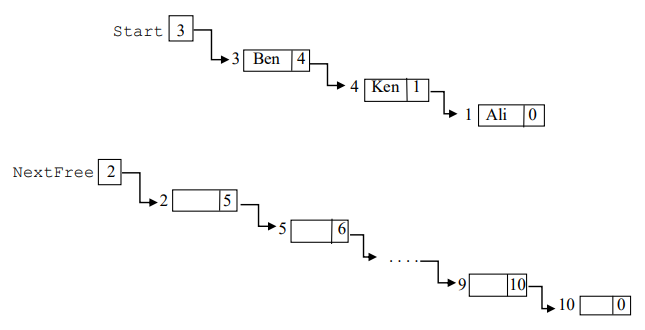
\includegraphics[width=0.65\paperwidth]{static/img/9597-HCI-2018-P1-Q3-1}
\par\end{center}

The diagram shows the linked list after the following sequence of
commands have been executed. 

\noindent\begin{minipage}[t]{1\columnwidth}%
\texttt{Create() }

\texttt{Insert('Ali', 1) }

\texttt{Insert('Jack', 1)}

\texttt{Insert('Ben',2)}

\texttt{Delete(1) }

\texttt{Insert('Jane', 2) }

\texttt{Insert('Ken', 3)}

\texttt{Delete(2)}%
\end{minipage}

The program to implement this ADT will use the classes \texttt{ListNode}
and \texttt{LinkedList} as follows: 
\begin{center}
\begin{tabular}{|l|}
\hline 
\hspace{0.25\columnwidth}\texttt{ListNode}\tabularnewline
\hline 
\texttt{Name : STRING}\tabularnewline
\texttt{Pointer : INTEGER}\tabularnewline
\hline 
\texttt{Constructor()}\tabularnewline
\texttt{SetName(Name:STRING)}\tabularnewline
\texttt{SetPointer(Pointer:INTEGER)}\tabularnewline
\texttt{GetName():STRING}\tabularnewline
\texttt{GetPointer():INTEGER}\tabularnewline
\hline 
\end{tabular}
\par\end{center}

\begin{center}
\begin{tabular}{|l|}
\hline 
\hspace{0.25\columnwidth}\texttt{LinkedList}\tabularnewline
\hline 
\texttt{Node : ARRAY {[}1..10{]} OF ListNode}\tabularnewline
\texttt{Start : INTEGER NextFree : INTEGER}\tabularnewline
\hline 
\texttt{Constructor()}\tabularnewline
\texttt{Insert (name: STRING, position: INTEGER)}\tabularnewline
\texttt{Delete (position: INTEGER)}\tabularnewline
\texttt{Length (): INTEGER}\tabularnewline
\texttt{IsEmpty(): BOOLEAN}\tabularnewline
\texttt{IsFull() : BOOLEAN}\tabularnewline
\hline 
\end{tabular}
\par\end{center}

\subsection*{Task 3.1 }

Write program code to define the classes \texttt{ListNode} and \texttt{LinkedList}. 

\subsection*{Evidence 15}

Program code for the \texttt{ListNode} and \texttt{LinkedList} classes.
\hfill{}{[}18{]}

\subsection*{Task 3.2 }

A method \texttt{Display()} is to be added, which displays the value
of \texttt{Start}, the value of \texttt{NextFree} and the contents
of \texttt{Node} array in index order. Write program code to implement
this method.

\subsection*{Evidence 16}

Your program code for Task 3.2. \hfill{}{[}4{]}

\subsection*{Task 3.3 }

Write code to create a \texttt{LinkedList} object in the main program.
Paste the sequence of commands in \texttt{COMMANDS.txt} into your
program code. Your program will then call the \texttt{Display} method. 

Execute your program to test it.

\subsection*{Evidence 17 }

Screenshot showing the output from running the program in Task 3.3.
\hfill{}{[}2{]}

A linear queue is implemented using the \texttt{LinkedList} class
as a super class. 

The subclass \texttt{Queue} has the following methods: 
\begin{itemize}
\item \texttt{Enqueue(item)} -{}- inserts item at the rear of the queue;
\item \texttt{Dequeue()} -{}- deletes the item at the front of the queue; 
\item \texttt{Display()} -{}- displays the contents of the queue using the
format given below.
\noindent \begin{center}
\texttt{}%
\begin{tabular}{lcl}
\texttt{Steven} & \texttt{$\leftarrow$} & \texttt{Front}\tabularnewline
\texttt{Celine} &  & \tabularnewline
\texttt{Tom} &  & \tabularnewline
\texttt{Ryan} & \texttt{$\leftarrow$} & \texttt{Rear}\tabularnewline
 &  & \tabularnewline
\multicolumn{3}{l}{\texttt{Numbers in queue : 4}}\tabularnewline
\end{tabular}
\par\end{center}
\end{itemize}

\subsection*{Task 3.4 }

Write program code for the subclass \texttt{Queue}.

Use appropriate inheritance and polymorphism in your design. 

\subsection*{Evidence 18}

Your program code for Task 3.4. \hfill{} {[}5{]}

\subsection*{Task 3.5 }

Write program code to: 
\begin{itemize}
\item create a new queue and add the data in the file \texttt{NAMES.txt}
to the queue 
\item remove two items from the queue 
\item display final contents of the queue 
\end{itemize}

\subsection*{Evidence 19 }

Your program code for Task 3.5. \hfill{} {[}2{]}

\subsection*{Evidence 20}

Screenshot showing the output from running the program in Task 3.5.
\hfill{} {[}1{]}